\begin{frame}{Explainable AI (XAI)}
	\centering
	\begin{tikzpicture}
		\visible<1>{\node[] (i1) at (0,0) {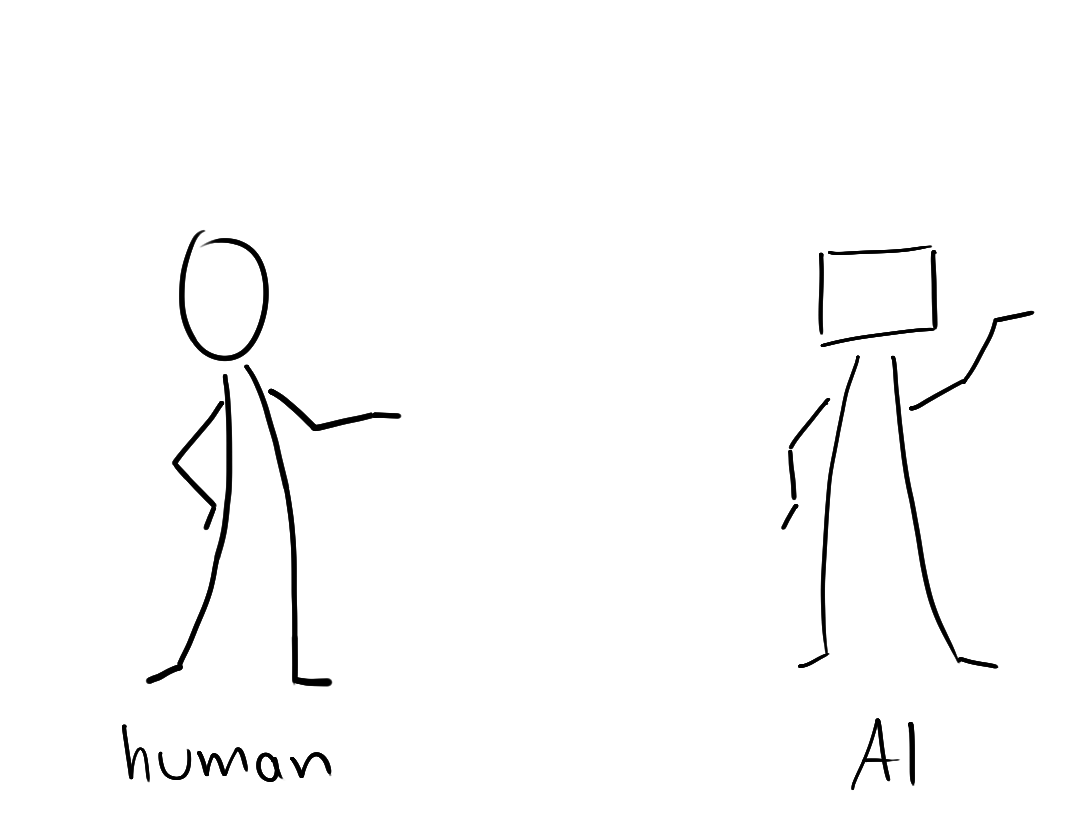
\includegraphics[scale=0.25]{images/intro1.png}};}
		\visible<2>{\node[] (i2) at (0,0) {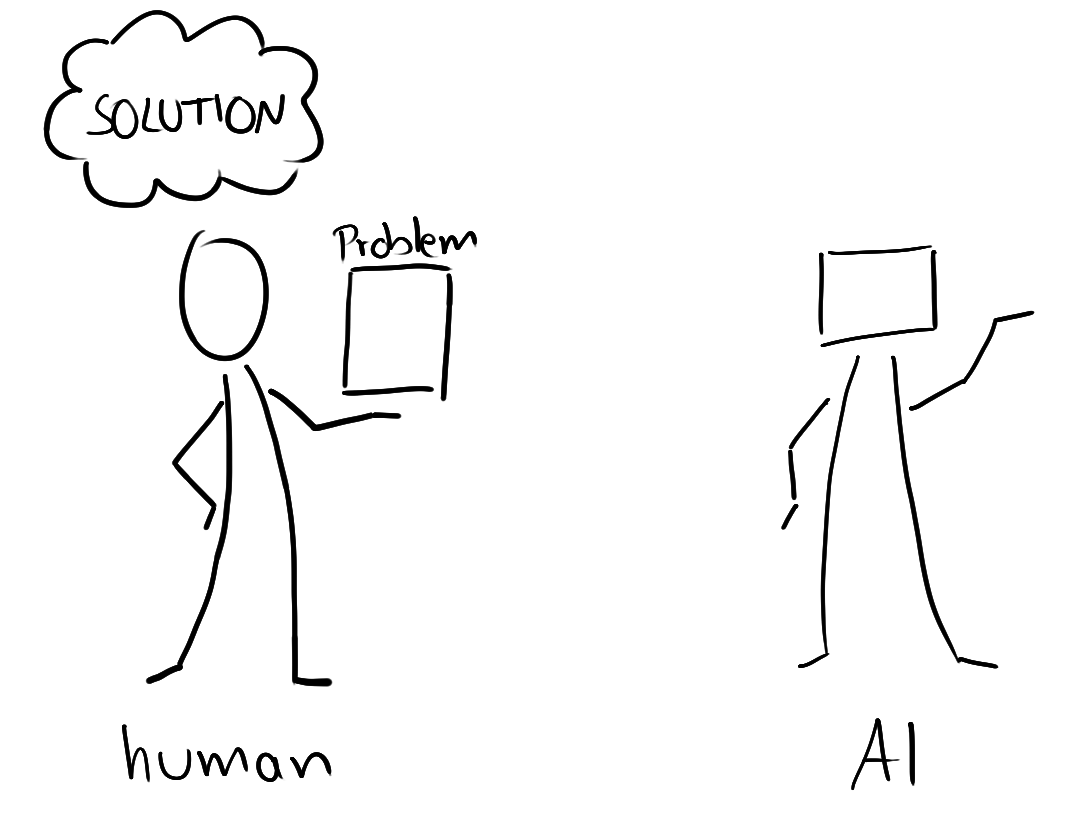
\includegraphics[scale=0.25]{images/intro2.png}};}
		\visible<3>{\node[] (i3) at (0,0) {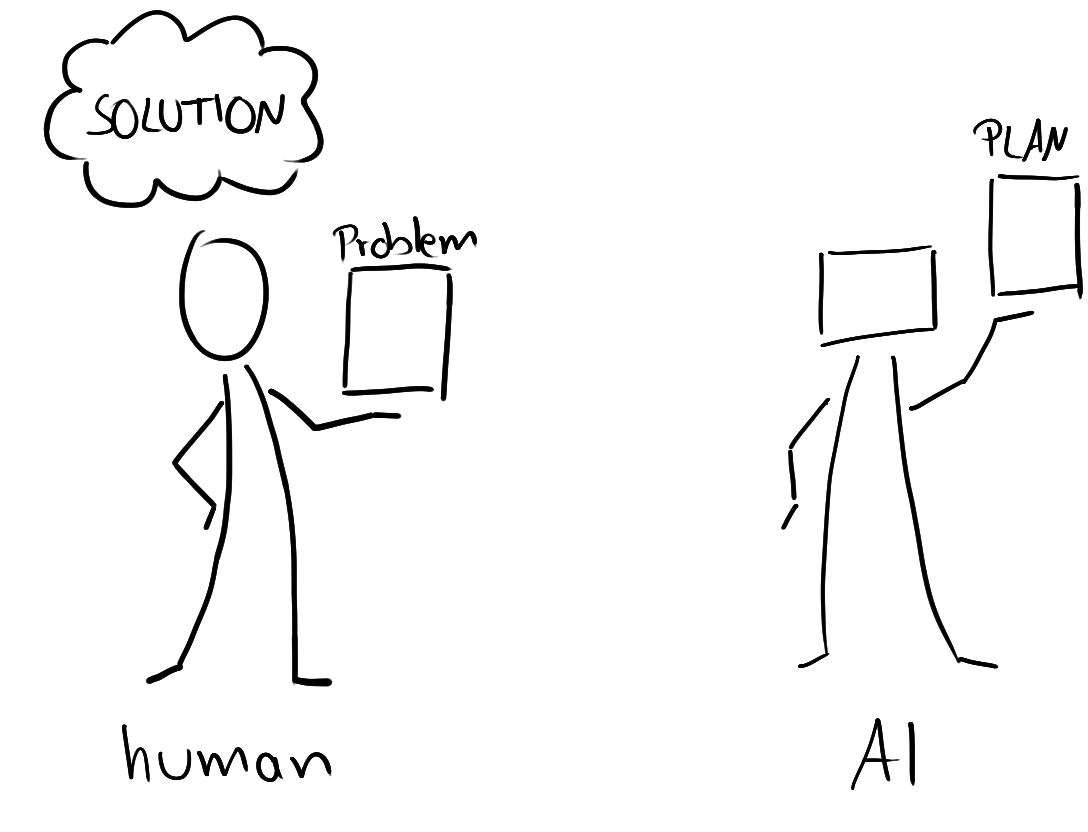
\includegraphics[scale=0.25]{images/intro3.png}};}
		\visible<4>{\node[] (i4) at (0,0) {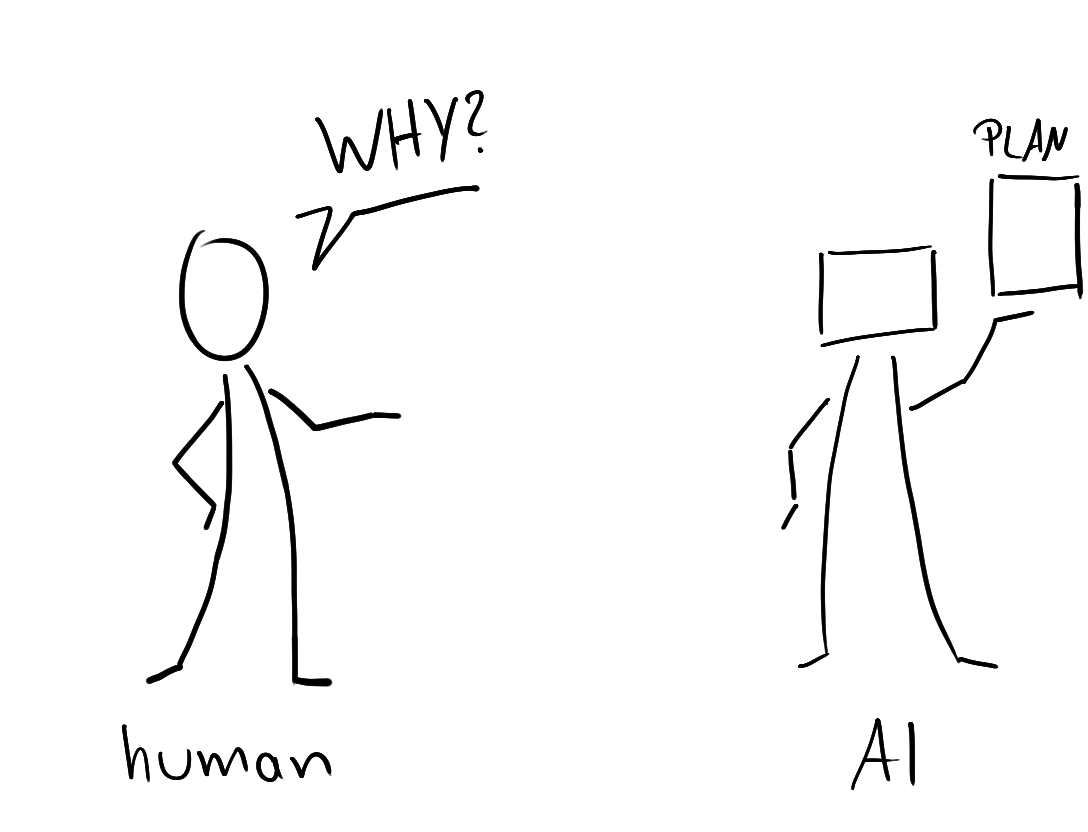
\includegraphics[scale=0.25]{images/intro4.png}};}
		\visible<5>{\node[] (i5) at (0,0) {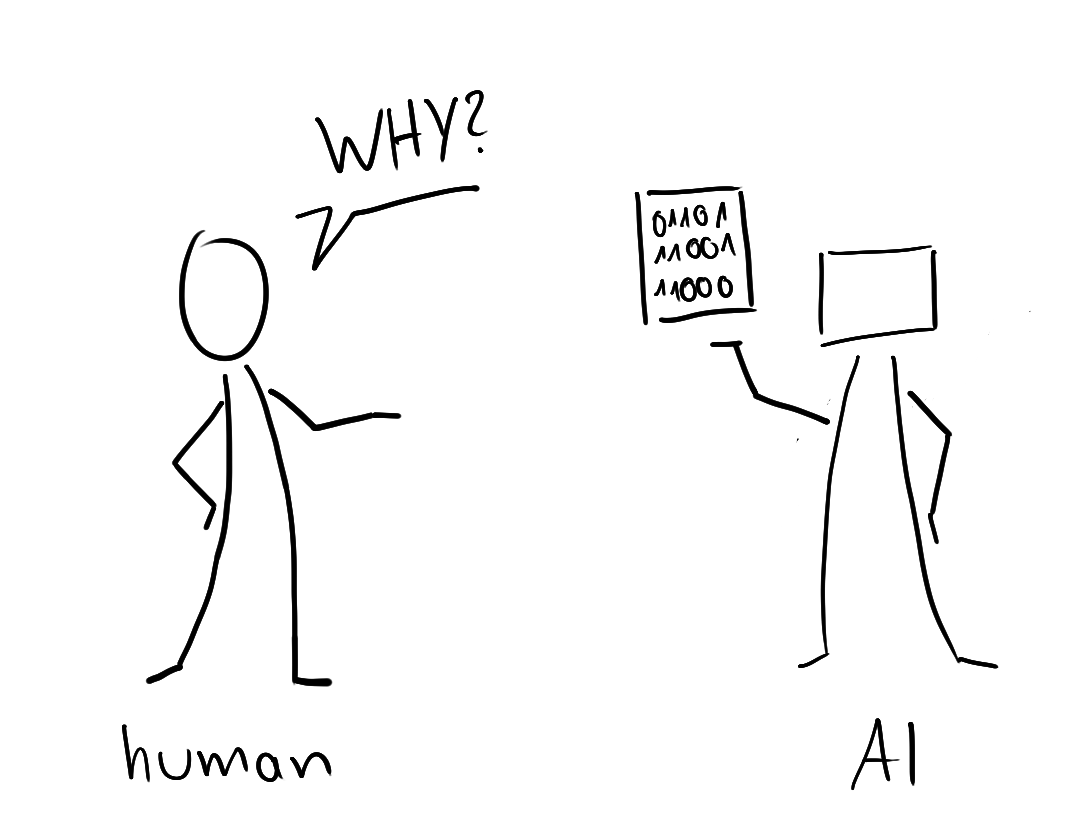
\includegraphics[scale=0.25]{images/intro5.png}};}
		\visible<6>{\node[] (i6) at (0,0) {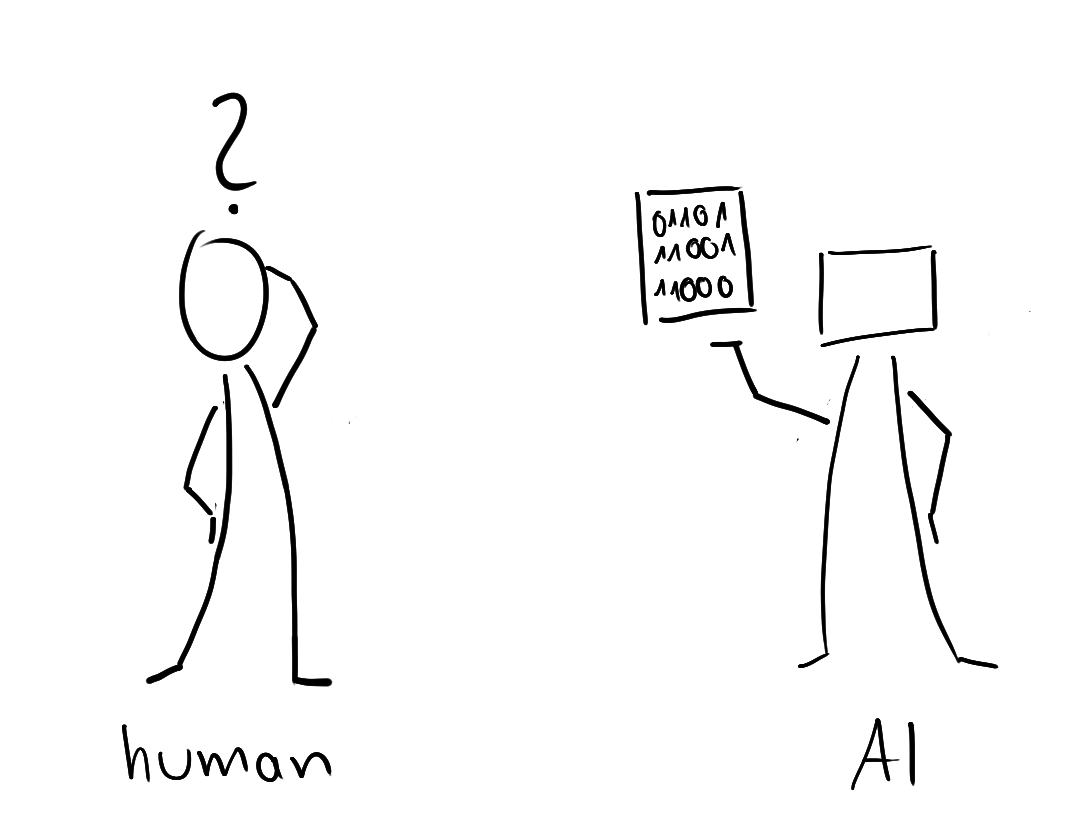
\includegraphics[scale=0.25]{images/intro6.png}};}
		%\visible<7>{\node[] (i7) at (0,0) {
\includegraphics[scale=0.25]{images/intro7.png}};}
		%\visible<8>{\node[] (i8) at (0,0) {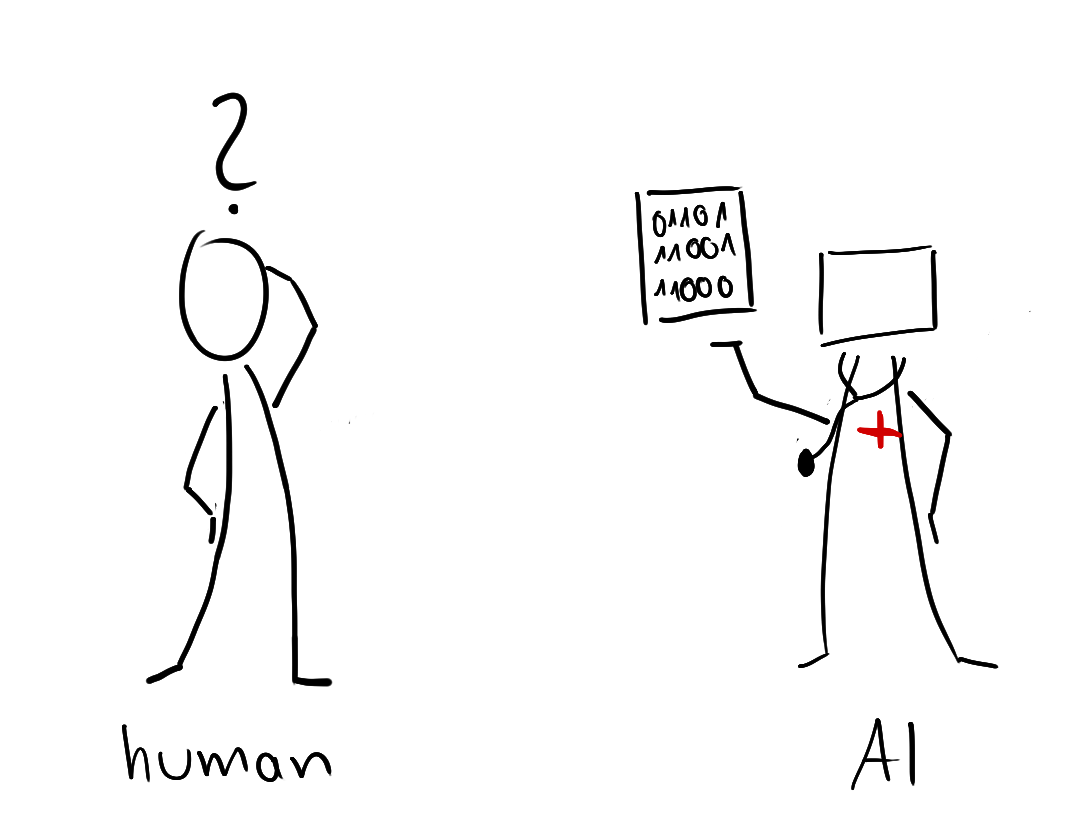
\includegraphics[scale=0.25]{images/intro8.png}};}
	\end{tikzpicture}\\
\end{frame}

\begin{frame}{Example}
	\centering
	\begin{tikzpicture}
		\visible<2->{
			\node[] (r1) at (1.5,2) {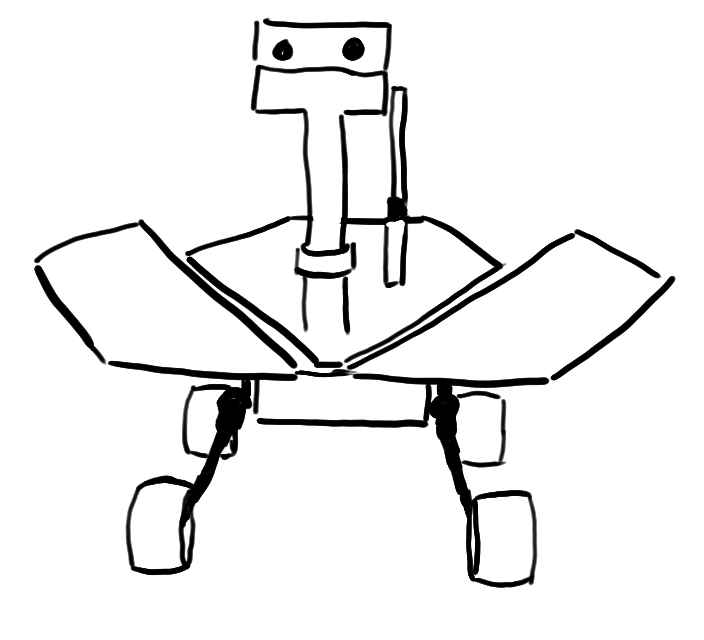
\includegraphics[scale=0.07]{images/rover2.png}};
			\node[] (b1) at (0.5,2.5) {
\includegraphics[scale=0.07]{images/battarie.png}};
			\node[] (r2) at (-5,-2.5) {
\includegraphics[scale=0.07]{images/rover1.png}};
			\node[] (b2) at (-5,-3.5) {
\includegraphics[scale=0.07]{images/battarie.png}};

			\node[] (m) at (0,0) {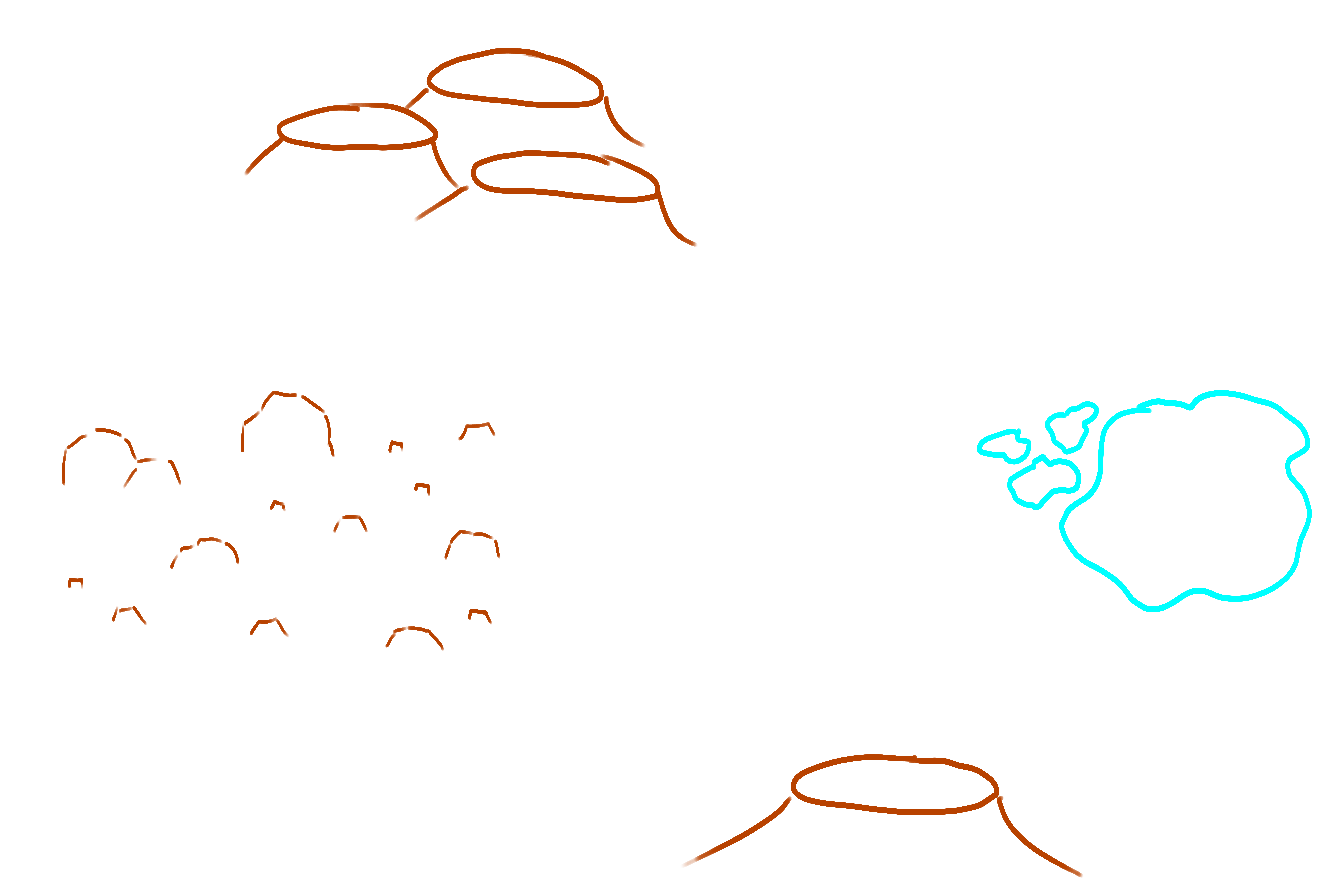
\includegraphics[scale=0.2]{images/mars_new.png}};
		}

		\visible<4->{
			\node[draw, circle, inner sep=3pt] (l1) at (-3,-3) {$L_1$};
			\node[draw, circle, inner sep=3pt] (l2) at (-2.1,1.3) {$L_2$};
			\node[draw, circle, inner sep=3pt] (l3) at (-0.5,-1) {$L_3$};
			\node[draw, circle, inner sep=3pt] (l4) at (3,2) {$L_4$};
			\node[draw, circle, inner sep=3pt] (l5) at (1.8,0) {$L_5$};
			\node[draw, circle, inner sep=3pt] (l6) at (3.2,-2.5) {$L_6$};

			\draw[thick] (l1) to (l2);
			\draw[thick] (l1) to (l3);
			\draw[thick] (l2) to (l3);
			\draw[thick] (l3) to (l5);
			\draw[thick] (l4) to (l5);
			\draw[thick] (l4) to (l6);
			\draw[thick] (l5) to (l6);
		}

		\visible<3->{
			\node[] (g) at (-1.9,-4) {\Large \textbf{goal}:};
			\node[] (i1) at (-0.5,-4) {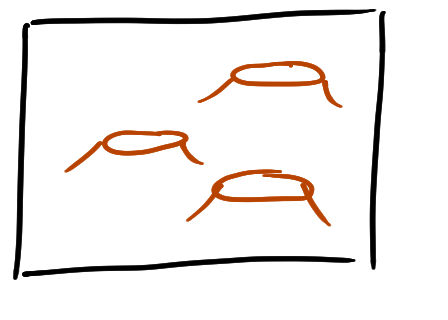
\includegraphics[scale=0.1]{images/image1.png}};
			\node[] (i2) at (0.8,-4) {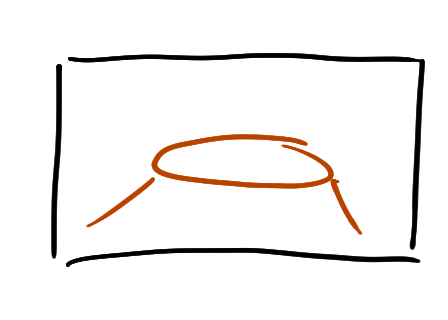
\includegraphics[scale=0.1]{images/image2.png}};
			\node[] (i3) at (2.5,-4) {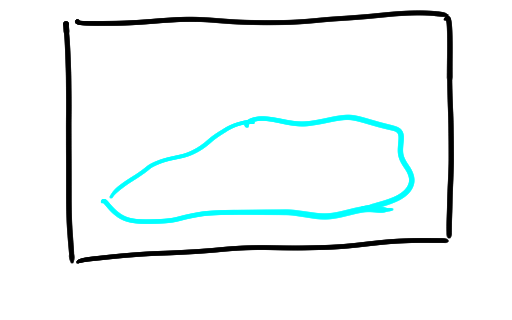
\includegraphics[scale=0.1]{images/image3.png}};
			\node[] (i1) at (-0.5,-4.6) {$I_1$};
			\node[] (i2) at (0.8,-4.6) {$I_2$};
			\node[] (i3) at (2.5,-4.6) {$I_3$};
		}

		\visible<5->{
			\node[align=left] (actions) at (-5,2) {
				%\Large \textbf{actions}:\\
				%\vspace*{0.2cm}
				\begin{varwidth}{3.5cm}
				\begin{itemize}
					\item<5-> $drive(R_i,L_x,L_y)$
					\item<6-> $takeImage_i(R_i)$
					%\item<7-> $send(R_i,I_i)$
				\end{itemize}
				\end{varwidth}
			};
		}
	\end{tikzpicture}
	
\end{frame}

%\begin{frame}{Planning Framework}
% actions, initial state, goal
%TODO do I need this
%\begin{itemize}
%	\item<1-> \textbf{variables}: $R_1, R_2, I_1, I_2, I_3$\\
%		domains: $R_i : \{L_1, ..., L_6\}$ $I_i : \{N, R_1, R_2, GS\}$
%	\item<2-> \textbf{actions}:
%		\begin{itemize}
%			\item $drive(R,L_x,L_y)$
%				\begin{itemize}
%					\item precondition: $R = L_x$
%					\item effect: $R = L_y$
%				\end{itemize}
%			\item $takeImage(R,I,L)$
%			\item $send(R,I)$
%		\end{itemize}
%		%TODO pre and effect
%	\item<3-> \textbf{initial state}: $I_i = N$, $R_1 = L_1$, $R_2=L_4$ 
%	\item<4-> \textbf{goal}: $I_i = GS$,	
%	\item<5-> \textbf{cost function}
	%\item \textbf{cost bound}

%\end{itemize}
%\end{frame}







